\documentclass[15pt]{article}
\usepackage[utf8]{inputenc}
\pagestyle{plain}
\usepackage[
top    = 2.75cm,
bottom = 2.55cm,
left   = 3.00cm,
right  = 3.00cm]{geometry}
\usepackage{graphicx}
\usepackage{xcolor}
\usepackage{hyperref}
\usepackage{titlesec}
\usepackage{tocloft}
\usepackage{caption}
\usepackage{subcaption}
\usepackage[none]{tocbibind}
\usepackage{float}
\usepackage{fancyhdr}

\titleformat*{\subsection}{\normalfont}
\graphicspath{ {./HS101 images/} }
\definecolor{- }{RGB}{245,92,71}
\definecolor{green}{RGB}{144,217,130}
\setcounter{secnumdepth}{5}
\setcounter{tocdepth}{1}

\pagestyle{fancy}
\fancyhf{}
\renewcommand{\headrulewidth}{0pt}
\renewcommand{\footrulewidth}{0.4pt}
\fancyfoot[R]{ADI}
\fancyfoot[L]{\thepage}

\renewcommand{\b}[1]{\begin{#1}}
\newcommand{\e}[1]{\end{#1}}
\renewcommand{\i}{\item{}}
\newcommand{\tb}[1]{\textbf{#1}}
\renewcommand{\thefigure}{}
\renewcommand{\cfttoctitlefont}{\Huge}

\b{document}
   \b{center}
       \vspace*{12cm}
       \tb{{\Huge EE214 {\color{- }boring} Short Notes}}
       
       \vspace{0.9cm}
       \tb{\LARGE Aditya Byju}
            
       \vspace{0.5cm}
       \large {\tb{Course Professor:} Prof. D. K. Sharma, Prof. Mariam Shojaei Baghini\\
       \tb{Ref:} Prof's video lectures\\
       \tb{Remark:} If you ain't getting anything, we'll be best friends!}
       
       \vspace{0.5cm}
       \tb{Digital Circuits Lab}
       
       \vspace{0.5cm}
       September 2021
            
       \vspace{0.8cm}
    \e{center}
\thispagestyle{empty}

\newpage
\tableofcontents
\addtocontents{toc}{\vspace{0.2cm}}

\newpage
\phantomsection
\section*{\color{- }Introduction}
\addcontentsline{toc}{section}{\large\color{- }Introduction}

\b{itemize}
    \i \tb{ceramic capacitors} - a type of low capacitance capacitors that have no polarity
    \i \tb{electrolytic capacitors} - these type of capacitors have higher capacitance values than ceramic capacitors and they do have polarity
    \begin{figure}[H]
    \centering
    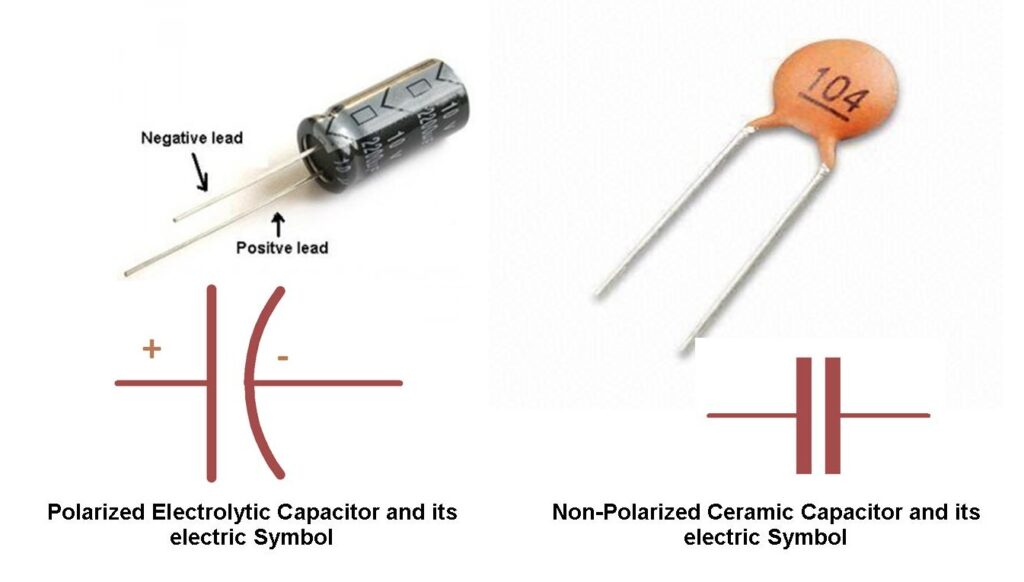
\includegraphics[width=11cm]{EE214 images/Electrolytic and ceramic capacitors.jpg}
    \end{figure}
    \i Single-turn and multi-turn potentiometers are variable resistances, also multi-turn potentiometers provide finer tuning of resistances
    \i \tb{hardware description language (HDL)} - is a specialized computer language used to describe the structure and behaviour of electronic circuits, and most commonly, digital logic circuits
    \i Very High Speed Integrated Circuit HDL (VHDL) - is a hardware description language which uses the syntax of ADA
    \i Uses of HDL:
    \b{itemize}
        \item[$-$] For describing hardware  
        \item[$-$] As a modelling language
        \item[$-$] For simulation of hardware
        \item[$-$] For early performance estimation of system architecture
        \item[$-$] For synthesis of hardware
        \item[$-$] For fault simulation, test and verification of designs
    \e{itemize}
    \i \tb{entity} - represents a template for a hardware block, describing its interface with other modules in terms of input and output signals
    \i \tb{testbench} - includes the circuit being designed, blocks which apply test signals to it and those which monitor its output
    \i \tb{architecture} - describes how an entity operates. An architecture is always associates with an entity. There can be multiple architectures associated with an entity.
    \begin{figure}[H]
    \centering
    \begin{minipage}{.4\textwidth}
    \centering
    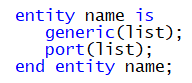
\includegraphics[width=.6\linewidth]{EE214 images/Entity declaration (VHDL 93 and later).png}
    \captionof{figure}{Entity declaration ($\geq$ VHDL 93)}
    \label{fig:test1}
    \end{minipage}%
    \begin{minipage}{0.7\textwidth}
    \centering
    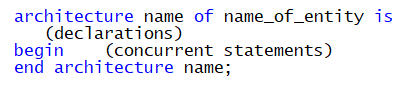
\includegraphics[width=.7\linewidth]{EE214 images/Architecture declaration (VHDL 93 and later).png}
    \captionof{figure}{Architecture declaration ($\geq$ VHDL 93)}
    \label{fig:test2}
    \end{minipage}
    \end{figure}
    \i The architecture inherits the port signals from its entity. Concurrent statements constituting the architecture can be placed in any order.
    \i Signals are carried by wires, variables are used for array indices, loop counters, etc.
    \i When you assign a value to a variable the assignment becomes effective immediately, however when you assign a value to a signal there is an associated delay for this assignment aas it is there in a real circuit
    \i \tb{component} - an {\color{green}entity $\leftrightarrow$ architecture} pair 
    \begin{figure}[H]
    \centering
    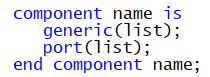
\includegraphics[width=4cm]{EE214 images/Component declaration (VHDL 93 and later).png}
    \caption{Component declaration ($\geq$ VHDL 93)}
    \end{figure}
    \i \tb{configuration} - describes linkages between component types and entity $\leftrightarrow$ architecture pairs
    \i Related declarations and design elements like subprograms and procedures can be placed in a {\color{green}package} for re-use. A package has a declarative part and an implementation part.
    \i Objects in a package can be referred to by a {\color{green}packagename.objectname} syntax 
    \i A description can include a {\color{green}use} clause to incorporate the package in the design. Objects in the package then becomes visible to the description without having to use the dot reference as above.
    \i Many design elements such as packages, definitions and entire entity $\leftrightarrow$ architecture pairs can be placed in a {\color{green}library}
    \i Any description invokes a library by first declaring it (For e.g. Library IEEE; )
    \i Objects in the library can then be incorporated in the design by a {\color{green}use} clause (For e.g. Use IEEE.std\_logic\_1164.all; )
    \i Various types of objects in VHDL are {\color{green}constants, variables, signals} and {\color{green}files.}
    \i Declaration of objects include their object type as well as the data type of values that they can acquire (For e.g. signal Enable: BIT; )
    \begin{figure}[H]
    \centering
    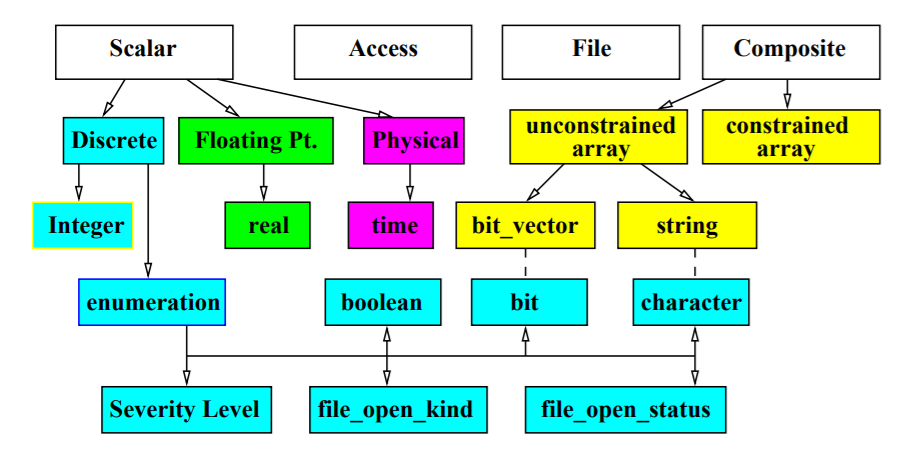
\includegraphics[width=11cm]{EE214 images/VHDL data types.png}
    \caption{VHDL Data types}
    \end{figure}
    \i VHDL {\color{green}enumeration types} allow us to define a set of values that a variable of this type can acquire. For example, we can define a data type by the following declaration:\\
    \hspace*{100pt}\tb{type} instr \tb{is} (add, sub, adc, sbb, rotl, rotr);
    \i Enumeration types pre-defined in the language are:
    \b{itemize}
        \item[$-$] \tb{type} bit \tb{is} (`0', `1');
        \item[$-$] \tb{type} boolean \tb{is} (false, true);
        \item[$-$] \tb{type} severity\_level \tb{is} (note, warning, error, failure);
        \item[$-$] \tb{type} file\_open\_kind \tb{is} (read\_mode, write\_mode, append\_mode);
        \item[$-$] \tb{type} file\_open\_status \tb{is} (open\_ok, status\_error, name\_error, mode\_error);
        \item[$-$] In addition to the above types, the character type enumerates all the ASCII characters
    \e{itemize}
    \i \tb{std\_logic} - is a signal  which can take 1 of 9 possible values. It is defined by:\\
    \hspace*{90pt}\tb{type} std\_logic \tb{is} (`U', `X', `0', `1', `Z', `W', `L', `H', `-');
    \i Object which  are declared to be of {\color{green}Physical type,} carry a value as well as a unit. These are used to represent physical quantities such as time, resistance and capacitance. Time is the only physical type, which is pre-defined in the language. We can define other physical types when required.
    \i {\color{green}Composite data types} are collections of scalar types. VHDL recognizes records and arrays as composite data types. Records are like structures in C. Arrays are indexed collections of scalar types. 
    \i Arrays can be constrained or unconstrained:
    \b{itemize}
        \item[$-$] In constrained arrays, the type definition itself places bounds on index values
        \item[$-$] In unconstrained arrays, no bounds are placed on index values
    \e{itemize}
    \i VHDL defines two built-in types of arrays: 
    \b{itemize}
        \item[$-$] bit\_vector\\
        \hspace*{40pt}\tb{type} bit\_vector \tb{is array} (natural range \textless\textgreater) \tb{of} bit;
        \item[$-$] strings\\
        \hspace*{40pt}\tb{type} string\_vector \tb{is array} (positive range \textless\textgreater) \tb{of} character;
    \e{itemize}
\e{itemize}

\phantomsection
\section*{\color{- }Structural description in VHDL}
\addcontentsline{toc}{section}{\large\color{- }Structural description in VHDL}

\b{itemize}
    \i {\color{green}Structural style} describes a design in terms of components and their interconnections. Each component declares its ports and the type and direction of signals that it expects through them. 
    \i A purely structural architecture for an entity will consist of:
    \b{itemize}
        \item[$-$] {\tb{Component declarations:}} to associate component types with their port lists.
        \item[$-$] {\tb{Signal declarations:}} to declare the signals used.
        \item[$-$] {\tb{Component instantiations:}} to place component instances and to portmap their ports to signals. Signals can be internal or port signals declared by the entity.
        \item[$-$] {\tb{Configurations:}} to bind component types to entity $\leftrightarrow$ architecture pairs.
        \item[$-$] {\tb{Repetition grammar:}} for describing multiple instances of the same component type – for example, memory cells or bus buffers.
    \e{itemize}
    \i When we associate a component type with a previously defined entity $\leftrightarrow$ architecture pair, the chosen architecture could itself contain other components - and these components in turn would be associated with other entity $\leftrightarrow$ architecture pairs. This hierarchical association can be described by a standalone design unit called a {\color{green}configuration.}
    \begin{figure}[H]
    \centering
    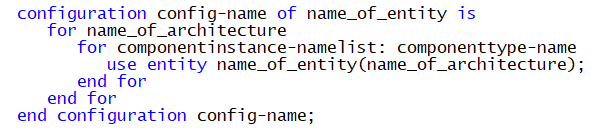
\includegraphics[width=11cm]{EE214 images/Simplified configuration construct.png}
    \caption{Simplified configuration construct}
    \end{figure}
    \i In VHDL, as we describe entities and architectures, these are compiled into a special library called {\color{green}work.} This library is always included and does not have to be declared.
\e{itemize}

\phantomsection
\section*{\color{- }File I-O in VHDL}
\addcontentsline{toc}{section}{\large\color{- }File I-O in VHDL}

\b{itemize}    
    \i In VHDL, in order to use files, we use a two step procedure:
    \b{itemize}
        \item[$-$] We declare a file type first. This associates a file type with the kind of objects that files of this type will contain.
        \item[$-$] We can then declare files of this file type. The file declaration associates a VHDL filename with a file type and optionally, with a Physical file name and file mode (read, write or append).
    \e{itemize}
    \i File type declaration:\\
    \hspace*{50pt}\tb{type} FileType \tb{is file of} DataType;
    \i If a file has not been opened during its declaration, it can be opened later by specific statements
    \i Opening files:\\
    \hspace*{50pt}\tb{procedure file\_open}(\tb{file} f: FileType;\\
    \hspace*{70pt} Phys\_name: in string;\\
    \hspace*{70pt} open\_kind: in file\_open\_kind:=read\_mode);
    \i Closing files:\\
    \hspace*{50pt}\tb{procedure file\_close}(\tb{file} f: FileType);
    \i Reading from files:\\
    \hspace*{50pt}\tb{procedure read}(\tb{file} f: FileType; value: out Data\_type);
    \i Writing to files:\\
    \hspace*{50pt}\tb{procedure write}(\tb{file} f: FileType; value: in Data\_type);
\e{itemize}

\phantomsection
\section*{\color{- }Behavioural description in VHDL}
\addcontentsline{toc}{section}{\large\color{- }Behavioural description in VHDL}

\b{itemize}
    \i Behavioural style describes a design in terms of its behaviour, and not in terms of a netlist of components. We describe behaviour through ``if-then-else” type of constructs, loops, sequential and concurrent assignment statements. Statements like “if-then-else” are inherently sequential. These must therefore occur only inside sequential bodies like processes.
    \i A concurrent assignment can be made conditionally by using `when’ clauses:\\
    \hspace*{50pt}name \textless= [delay-mechanism]\\
    \hspace*{70pt}waveform \tb{when} Boolean-expression \tb{else}\\
    \hspace*{70pt}waveform \tb{when} Boolean-expression;
    \i VHDL operators:
    \b{itemize}
        \item[$-$] \tb{Logical operators:} AND, OR, NAND, NOR, OR, XNOR and NOT
        \item[$-$] \tb{Relational operators:} =, /, \textless, \textless=, \textgreater, \textgreater=
        \item[$-$] \tb{Shift operators:} SLL (logical left), SLA (arithmetic left) SRL (logical right), SRA (Arithmetic right), ROL (rotate left) and ROR (rotate right)
    \e{itemize}
    \i Sequential constructs need to be placed inside a process. A process uses the syntax:\\\\
    \hspace*{50pt} [process-label:] \tb{process} [(sensitivity-list)][\tb{is}]\\
    \hspace*{50pt} [declarations]\\
    \hspace*{50pt} \tb{begin}\\
    \hspace*{70pt} [sequential statements]\\
    \hspace*{50pt} \tb{end process} [process-label];\\\\
    Sequential statements include ``if” constructs, case statements, looping constructs, assertions, wait statements etc.
\e{itemize}

\phantomsection
\section*{\color{- }JTAG and Scanchain}
\addcontentsline{toc}{section}{\large\color{- }JTAG and Scanchain}
\tb{JTAG:}
\b{itemize}
    \i Joint Test Action Group
    \i Industry standard for verifying designs and testing PCBs
    \i Connects to an on-chip Test Access Port (TAP) controller
    \i TAP controller implements a protocol to access a set of registers or pins of a system
    \i Response is then stored into Flip-Flops and then compared with a golden response
\e{itemize}
\tb{Scanchain:}
\b{itemize}
    \i Scan chain is a technique used in design for testing. The objective is to make testing easier by providing a simple way to set and observe every flip-flop in an IC. 
\e{itemize}



\e{document}